\subsection{Third Experience}

\subsubsection{DNS tracing with Wireshark --- Browsing}
To see how Wireshark displays DNS requests, we opened our browser and visited
the following pages:

\begin{itemize}
    \item www.ietf.org
    \item www.google.com
    \item www.cisco.com
    \item www.utec.edu.pe
\end{itemize}

We then saw that Wireshark uses the following structure to display DNS
requests:

\begin{figure}[htbp]
    \centering
    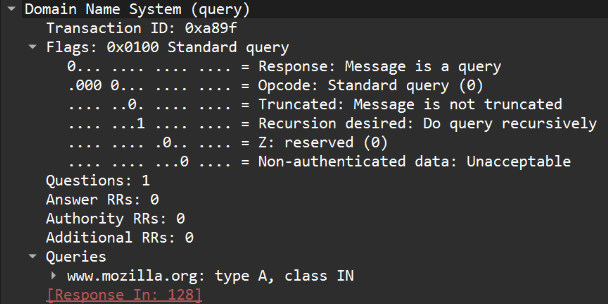
\includegraphics[width=1\linewidth]{img/13.png}
    \caption{Wireshark DNS request}\label{fig:13}
\end{figure}

\begin{itemize}
    \item TXID:\@ Used as a unique id to validate correctness (UDP skill issue)
    \item Flags: Used to indicate message type (query/response), opcode (many types),
          truncated (if too large, use TCP), recursion (recursion or sequential), Z
          (unused, always 0)
    \item Answer RRs: Resource records attached to query (0 since is query)
    \item Authority RRs: Similar to above, but for authority servers
    \item Additional RRs: Similar to above, but for additional records
\end{itemize}

The query contains the requested hostname, type A means it's asking for the IP
address. Class IN is apparently the standard used by most queries.

We then wanted to see which DNS servers were used when making the request.
Wireshark's top window contains this information. As expected, the DNS server
used for the queries were the university's DNS servers, and it contains no
answers, as it is a query.

\begin{figure}[htbp]
    \centering
    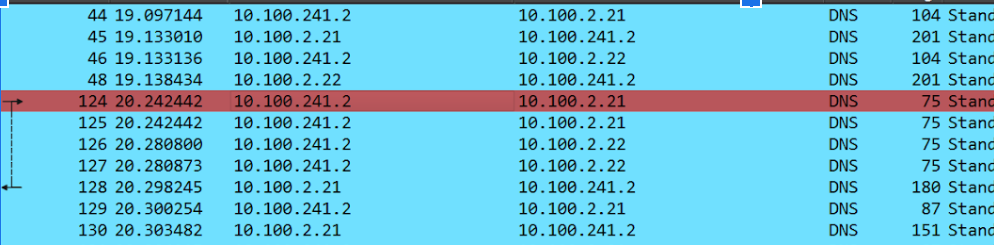
\includegraphics[width=1\linewidth]{img/14.png}
    \caption{Wireshark packet window}\label{fig:14}
\end{figure}

\subsubsection{DNS tracing with Wireshark --- nslookup}
For this subsection, we used \texttt{nslookup} tool to make a DNS query for the
hostname \textit{www.mit.edu}. Then, we selected the corresponding packets and
observered the packet details.

The destination port for the DNS query message is 53 (default DNS port), which
is also the source port of the response message.

\begin{figure}[htbp]
    \centering
    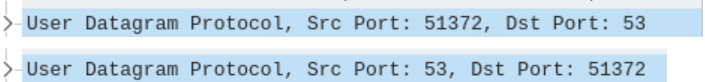
\includegraphics[width=1\linewidth]{img/15.png}
    \caption{Source and Destination Ports}\label{fig:15}
\end{figure}

We also saw that the DNS query message was sent to the university's DNS server,
which makes sense.

\begin{figure}[htbp]
    \centering
    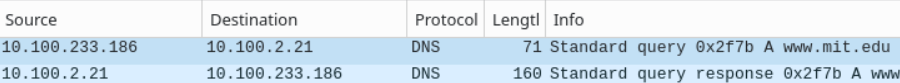
\includegraphics[width=1\linewidth]{img/16.png}
    \caption{DNS query destination address}\label{fig:16}
\end{figure}

Each DNS query has a type, which determines what kind of information is being
requested. In this case, the request's type is A, which means it sent a
hostname and requested an IP address. The message does not contain any answers,
as it is a query message.

\begin{figure}[htbp]
    \centering
    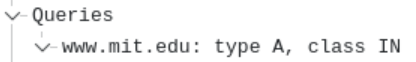
\includegraphics[width=1\linewidth]{img/17.png}
    \caption{DNS query type}\label{fig:17}
\end{figure}

After that, we examined the DNS response message, and it contained three
answers:

\begin{itemize}
    \item Answer 1: Canonical name of the requested hostname
    \item Answer 2: Canonical name of the CDN in use
    \item Answer 3: IP address of the previously obtained canonical name
\end{itemize}

\begin{figure}[htbp]
    \centering
    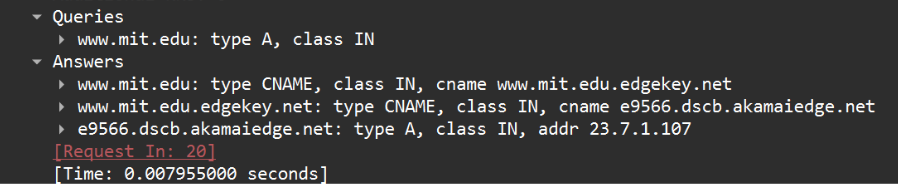
\includegraphics[width=1\linewidth]{img/18.png}
    \caption{DNS response answers and types}\label{fig:18}
\end{figure}

We then repeated the same process, but setting the query type to NS, which asks
for the authoritative servers for the domain. As expected, the DNS query
message was sent to the local DNS server.

\begin{figure}[htbp]
    \centering
    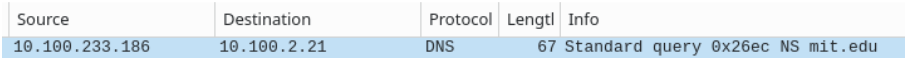
\includegraphics[width=1\linewidth]{img/19.png}
    \caption{NS destination address}\label{fig:19}
\end{figure}

Further examining the query message reveals that its type is NS, as we
intended, and it doesn't contain any answers yet, as it is a query message.

\begin{figure}[htbp]
    \centering
    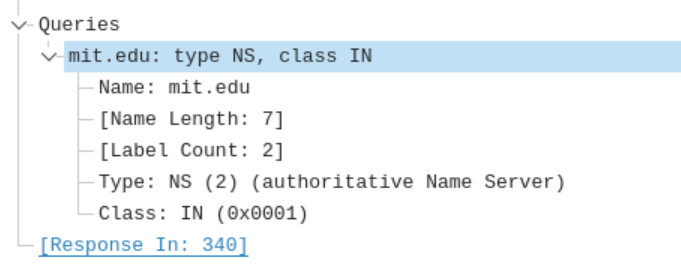
\includegraphics[width=1\linewidth]{img/20.png}
    \caption{DNS query message}\label{fig:20}
\end{figure}

We then selected the response message, which contained the IP addresses of
several MIT nameservers, as well as their IP addresses as additional records.

\begin{figure}[htbp]
    \centering
    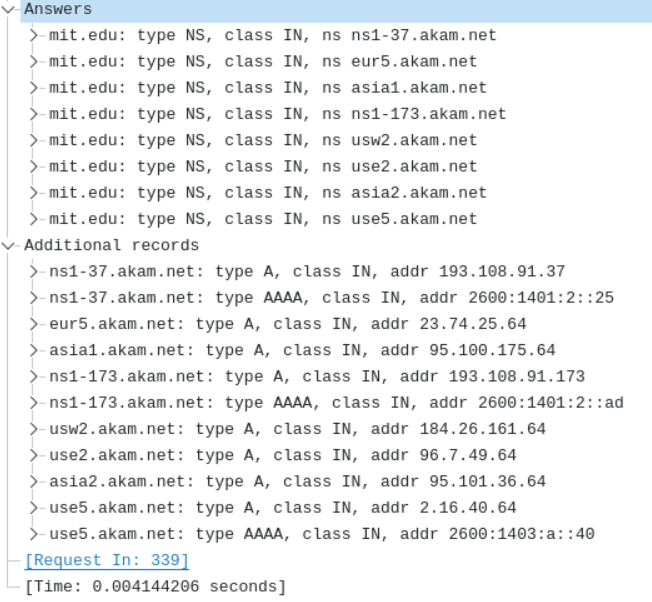
\includegraphics[width=1\linewidth]{img/21.png}
    \caption{DNS NS results}\label{fig:21}
\end{figure}

Finally, we repeated the experiment once more with a different command:
\texttt{nslookup www.aiit.or.kr bitsy.mit.edu}. This command request the IP
address of the hostname \textit{www.aiit.or.kr} but using the DNS server
\textit{bitsy.mit.edu}.

Checking the query message, we can see that the destination address is our
local DNS server's address.

\begin{figure}[htbp]
    \centering
    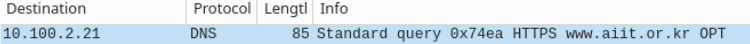
\includegraphics[width=1\linewidth]{img/22.png}
    \caption{DNS query destination address}\label{fig:22}
\end{figure}

The query itself does not contain any answers, as it is a query message, and is
of type HTTPS.\@

\begin{figure}[htbp]
    \centering
    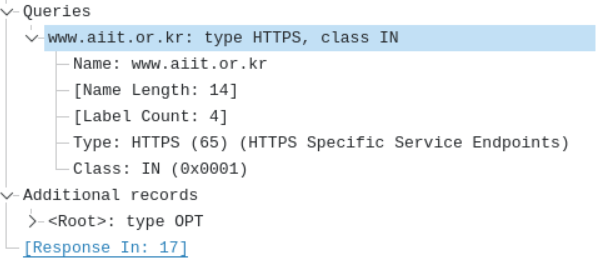
\includegraphics[width=1\linewidth]{img/23.png}
    \caption{DNS query type}\label{fig:23}
\end{figure}

This time, the query is not able to be resolved by the requested DNS server,
and it times out after a few attempts.

\begin{figure}[htbp]
    \centering
    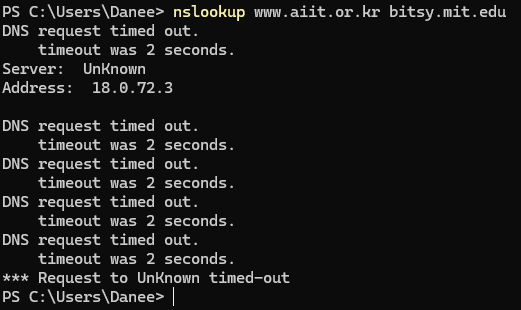
\includegraphics[width=1\linewidth]{img/24.png}
    \caption{nslookup timeout}\label{fig:24}
\end{figure}

This might be due to the MIT DNS server security policies, as it might not be
allowed to answer queries from outside its domain. Furthermore, it might only
be able to resolve hostnames outside its domain if the request came from a
device inside its network, probably as a security measure.